\appendix
%\chapter{Proof of Theorem 1}\label{appendix1}
\chapter{動作再現における観点推定の成否の判定}\label{appendix1}

動作の再現実験における、教示誤差と再現誤差の関係を図\ref{figure:errors}に示す。
%%%%%%%%%%%%%%%%%%%%%%%%%%%%%%%%%%%%%%%%%%%%%%%%%%%%%%%%%%%%%%%%%%%%%%%%%%%%%%%%%%%%%%%%%%%%%%%%%%%%%%%
	\begin{figure}
%中央ぞろえ
		\begin{center}
			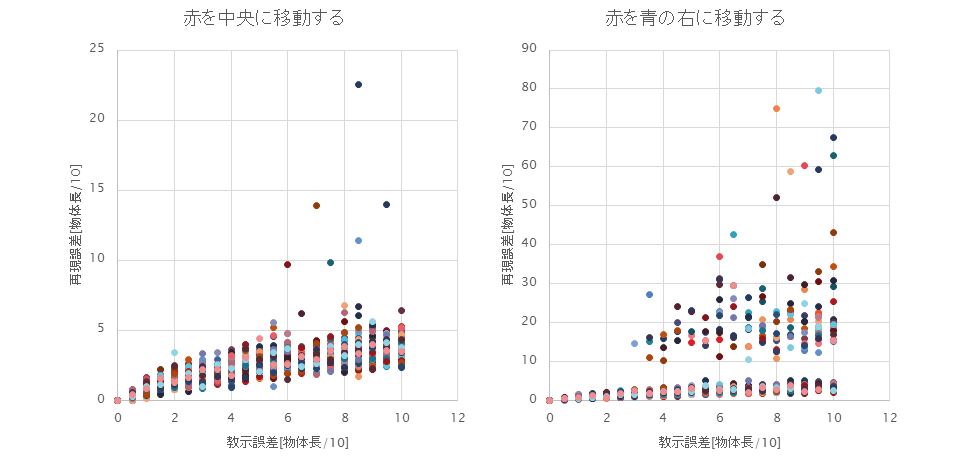
\includegraphics[width=15.5cm]{chart6.png} \\ %eXの基本として, \\ で緊急改行ができる。(今回の場合や行列などを除き、あまり使わない)
			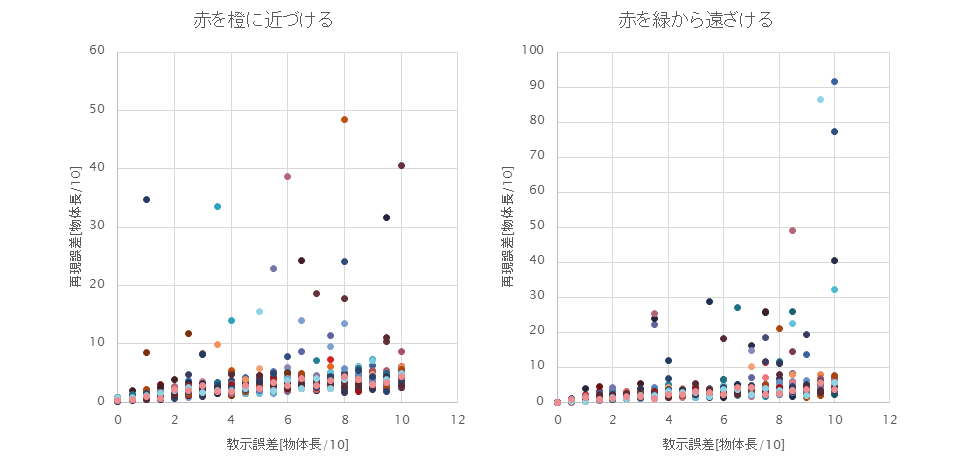
\includegraphics[width=15.5cm]{chart7.png} \\ %eXの基本として, \\ で緊急改行ができる。(今回の場合や行列などを除き、あまり使わない)
			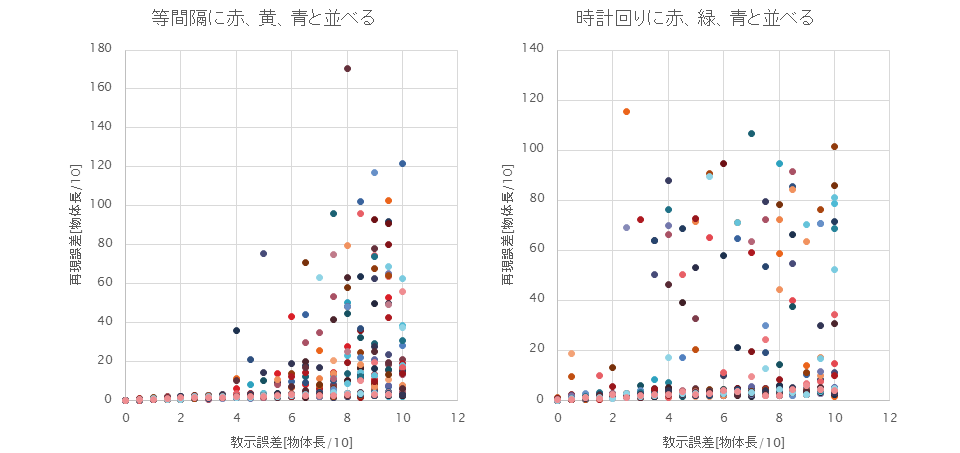
\includegraphics[width=15.5cm]{chart8.png} \\ %eXの基本として, \\ で緊急改行ができる。(今回の場合や行列などを除き、あまり使わない)
			\caption{教示誤差と再現誤差の関係}
			\label{figure:errors}
		\end{center}
	\end{figure}
%%%%%%%%%%%%%%%%%%%%%%%%%%%%%%%%%%%%%%%%%%%%%%%%%%%%%%%%%%%%%%%%%%%%%%%%%%%%%%%%%%%%%%%%%%%%%%%%%%%%%%%
ここで、横軸は教示誤差の分散、縦軸は再現誤差の標準偏差を表す。
教示動作から学習したモデルを用いた動作再現を行う際、教示動作自体に誤差が含まれている場合、一つ抜き法によるテスト時に使用するデータも教示動作の一つであるために必然的に誤差が生じる。そのため一つ抜き法により計算された再現誤差が教示誤差に依るものなのか誤学習に依るものなのかを区別する基準が必要である。ここでは正規分布から生成された誤差を含む教示動作から適切に学習された場合に再現誤差も正規分布に従うことを示し、正規分布の性質から観点推定の成否の基準値を設定する。
まず、適切な観点(原点となる参照点と座標系)からの$N$回分の各教示動作における目標位置を$Θ=\{θ_{1} , θ_{2} , \ldots , θ_{N}\}$に対し、$Θ$を用いた一つ抜き法による評価値を次のように求める。
	\begin{equation}
	\label{CrossVaridation}
Cr(Θ) = \frac{1}{N} \sum_{n=1}^{N} F(θ_{n} | Θ \backslash θ_{n})
\end{equation}
ここで\ref{CrossVaridation}式の右辺$F(θ_{n} | Θ \backslash θ_{n})$は、$θ_{n}$を除く$Θ$を用いて学習し再現を行った結果の目標位置と$θ_{n}$の誤差を表す。動作再現は選択された観点に割り当てられた正規分布の平均を出力するので、
\begin{equation}
\label{F}
F(θ_{n} | Θ \backslash θ_{n}) = |θ_{n} - mean(Θ \backslash θ_{n})| = |\frac{N}{N-1}(θ_{n} - mean(Θ))|
\end{equation}
である。ただし$mean(A)$はAの平均とする。\ref{F}式を\ref{CrossVaridation}に代入すると
\begin{equation}
\label{Cr2}
Cr(Θ) = \frac{1}{N} \sum_{n=1}^{N}  |\frac{N}{N-1}(θ_{n} - mean(Θ))|
 = \frac{N}{N-1}\frac{1}{N}  \sum_{n=1}^{N}  |(θ_{n} - mean(Θ))| 
\end{equation}
と整理できる。ここで\ref{Cr2}式の右辺$|(θ_{n} - mean(Θ))|$は$θ_{n}$の持つガウス誤差と等しいので、
\begin{equation}
\label{Cr3}
mean(Cr(Θ)) = \frac{N}{N-1} * mean(\frac{1}{N}  \sum_{n=1}^{N}  |(θ_{n} - mean(Θ))| )
 = _frac{N}{N-1} * mean(G_{error})
\end{equation}



%\chapter{Proof of Theorem 2}\label{appendix2}
%\chapter{定理2の証明}\label{appendix2}
